% Copyright (c) 2013 Datalogisk Kantineforening.
% Licenseret under EUPL, version 1.1 udelukkende.
% Licensteksten: https://joinup.ec.europa.eu/software/page/eupl/licence-eupl

\documentclass{article}

\usepackage[multi,landscape]{skiltefabrikken}


\begin{document}

\maketitle

\null

\begin{minipage}[l]{.5\textwidth}
  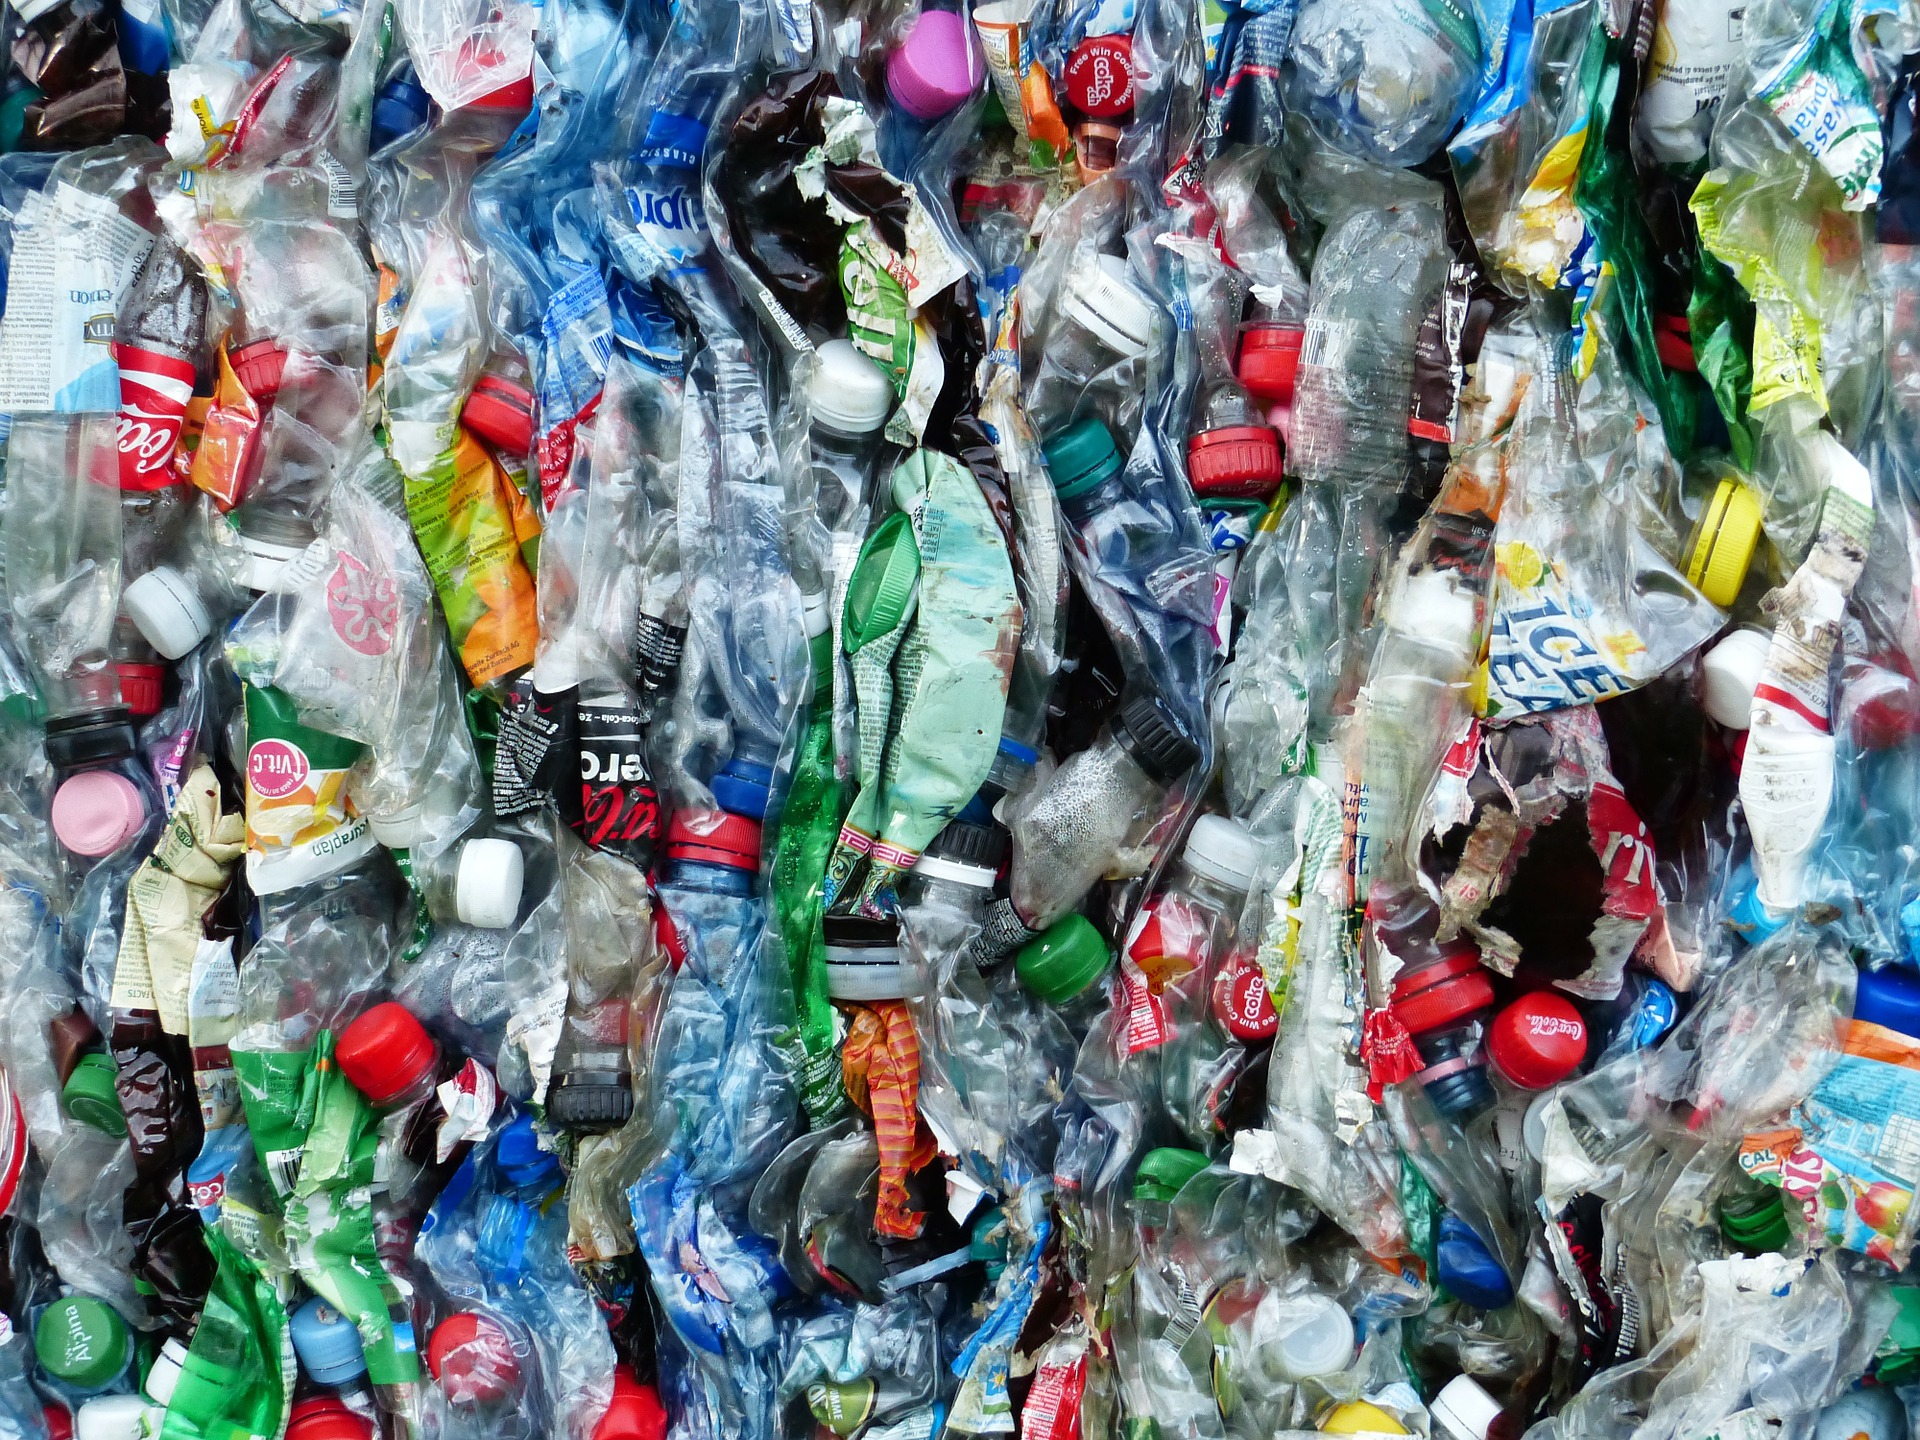
\includegraphics[width=12cm]{../billeder/plastik.jpg}
\end{minipage}
\begin{minipage}[c]{.5\textwidth}
\overskrift{KUN TIL PLASTIK}
\vspace{-0.7cm}

\Large Hvis spanden er fyldt så tag den med ned til affaldscontaineren ved Nørre
Allé.\\
\textbf{OBS!} Kig efter containeren til \underline{\textbf{plastik}}.

\english
\overskrift{ONLY FOR PLASTICS}
\vspace{-0.5cm}

\Large If the bucket is filled bring it with you to the container by Nørre Allé.
\textbf{NB!} Look for the container marked \underline{\textbf{plastik}}.
\end{minipage}

\dansk
\underskriv

\end{document}
